Below follows the results of the failure estimation as well as the estimation method used.

\subsection{TROPICO R-1500}
TROPICO R-1500 is a Brazilian Electronic Switching System with 1500 subscribers and a file, godata1.txt containing the failure count of said system, will be analyzed. A compliation of the results are found in Table~\ref{goelokumototable} below.
\subsubsection*{Subjective Estimation} 
First the cumulative sum of the faults found in week 1 to week 50 were plotted, see Figure~\ref{cumulativegodata1} below, to see if a failure over time trend could be found.
The inspectors identified an exponentially declining trend and estimated the two variables $N_{future}$ and $N_{tot}$ to be 500 and 600 faults respectively, see Table~\ref{goelokumototable}. 
\subsubsection*{Goel-Okumoto method}
To use the Goel-Okumoto method, described in section~\ref{methods}, a program, go.m, were used to calculate the variables $a=547.5$ and $b=0.0242$.
When estimating the $N_{future}$ variable the found values of $a$ and $b$ were inserted in the Goele-Okumoto formula and $t$ were increased to 75, since $N_{future}$ is the cumulative sum of the errors found in additionally 50\% time. 
$N_{tot} = a$ since it is the sum of all errors found in an infinite amounut of time.
The estimation of $N_{future}$ and $N_{tot}$ was 458.1 and 547.5 respecitvely, see Table~\ref{goelokumototable}.
\subsubsection*{Real Data}
To find the accuracy of the subjective estimation and the Goel-Okumoto method the real values of $N_{future}$ and $N_{tot}$ were found by using a file, godata2.txt, containing the failure count of 31 more weeks. 
The real value of $N_{future}$ is the sum of all errors up to weak 75, which gives $N_{future}=459$, which is very close to the estimated value of 458.1. $N_{tot}$ on the other hand cannot be verified since there is no, nor will it ever be, a file containing the errors found until infinity. However, the last value of godata2.txt is 461 and is found at week 81, compared to 468 at week 81 in the Goel-Okumoto estimation. Since this is within 1.5\% of the estimation, it will be assumed that Goel-Okumoto estimates the $N_{tot}$ good enough.

\begin{figure}[htb!]
\begin{center}
	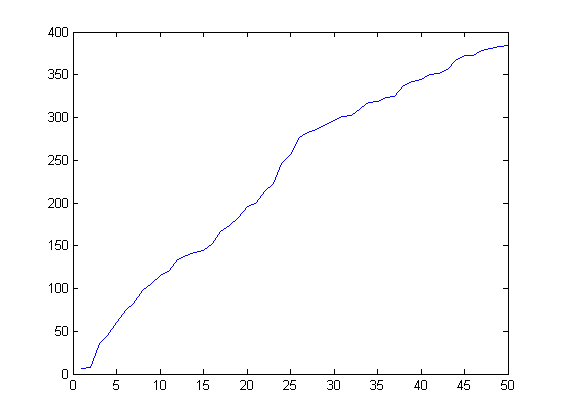
\includegraphics[width=0.5\textwidth]{cumsumgodata1plot.png}
\caption{The cumulative sum of failures found in TROPICO R-1500 in 50 weeks.}
\end{center}
\label{cumulativegodata1}
\end{figure}

\begin{table}[!htb]
	\centering
	\caption{$N_{future}$ and $N_{tot}$ with subjective and GO-estimation as well as real values.}
	\label{goelokumototable}	
    \begin{tabular}{|l|l|l|}
        \hline
        ~ & $N_{future}$ & $N_{tot}$ \\ \hline
        Subjective Estimation            & 500   & 600 		\\ 
        GO estimation                    & 458.1 & 547.5	\\ 
        Actual values                    & 459 	 & 461		\\ 
        \hline
    \end{tabular}
\end{table}

\subsection{Reliability Jelinski-Moranda}
In this excersice a file, jmdata1.txt, containing the failures found in a system as well as the time between them will be used.

\subsubsection*{Subjective Estimation} 
First te cumulative sum of the time between failures and the number of failures were plotted, see Figure~\ref{cumulativejmdata1} below. Here as well the inspectors identified an exponentially declining trend and estimated $N_{future}$ and $N_{tot}$ to be 230 and 500 respectively, see Table~\ref{jelinskimorandatable} below.

\subsubsection*{Jelinski-Moranda Estimation}
To use the Jalinski-Moranda method, described in section~\ref{methods}, a program, jm.m, were used to calculate the variables $N=226.5$ and $\phi=1.18\times10^{-4}$. Since Jelinski-Moranda estimates the intensity of failures $N_{future}$ cannot be estimated using this method.
$N_{tot}$ on the other hand is the fault when the JM method equals zero, because if the intensity of failures equals zero no new errors will occur, which gives $N_{tot}=226.5$.

\subsubsection*{Real Data}
To find the accuracy of the subjective estimation and the Jelinski-Moranda method the real values of $N_{future}$ and $N_{tot}$ were found by using a file, jmdata2.txt, containing additionally 57 more failures as well as the time between them. Since the end time in jmdata1.txt was arounud 9000 unit of time the $N_{future}$ is the number of faults found after 13500 units of time. By plotting the cumulative sum of the time between errors in jmdata2.txt it was found that the real value of $N_{future}=200$. The real data value of $N_{tot}$ is $N_{tot}=207$ and occurs at time 16656 and with an failure intensity $\lambda=0.0025$. Even tough this value is a bit of from the estimated $N_{tot}$ it is assumed to be realistic since according to the Jelinski-Moranda method the failure intensity $\lambda=0.0025$ at this point and Figure~\ref{cumulativejmdata2} shows that the amount of failures has severly stagnated at this point.



\begin{figure}[htb!]
\begin{center}
	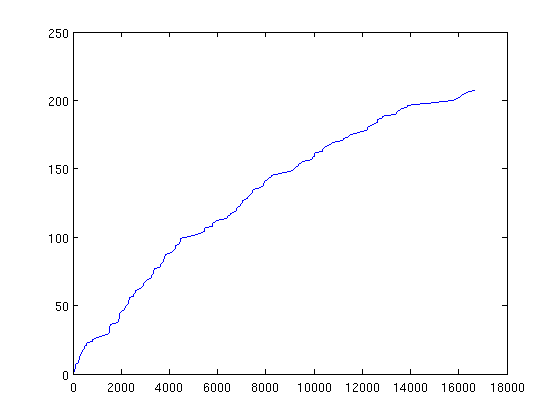
\includegraphics[width=0.5\textwidth]{cumsumjmdata2.png}
\caption{The cumulative sum of the time between failures as well as the failures found in an analyzed system.}
\end{center}
\label{cumulativejmdata2}
\end{figure}



\begin{figure}[htb!]
\begin{center}
	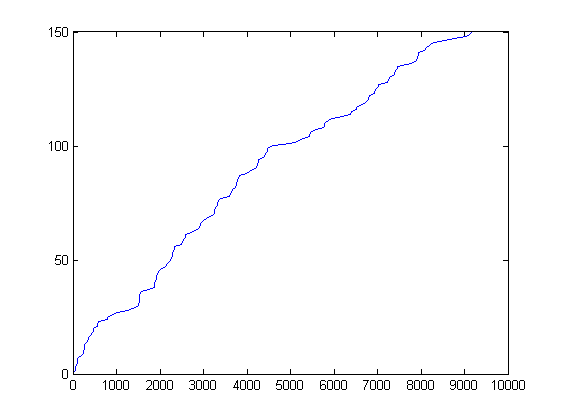
\includegraphics[width=0.5\textwidth]{cumsumjmdata1plot.png}
\caption{The cumulative sum of the time between failures as well as the failures found in an analyzed system.}
\end{center}
\label{cumulativejmdata1}
\end{figure}

\begin{table}[!htb]
	\centering
	\caption{$N_{future}$ and $N_{tot}$ with subjective and JM-estimation as well as real values.}
	\label{jelinskimorandatable}	
    \begin{tabular}{|l|l|l|}
        \hline
        ~ & $N_{future}$ & $N_{tot}$ \\ \hline
        Subjective Estimation            & 230   & 500 		\\ 
        JM estimation                    & N/A   & 226.5	\\ 
        Actual values                    & 200 	 & 207		\\ 
        \hline
    \end{tabular}
\end{table}